\documentclass{standalone}

\usepackage{tikz}
\usetikzlibrary{decorations.pathmorphing}
\tikzset{every node/.style={align=center}}
\tikzstyle{snake} = [decorate, decoration={snake, segment length=1mm, pre length = 1.5mm, post length = 1mm, amplitude=2mm}]

\begin{document}
	
	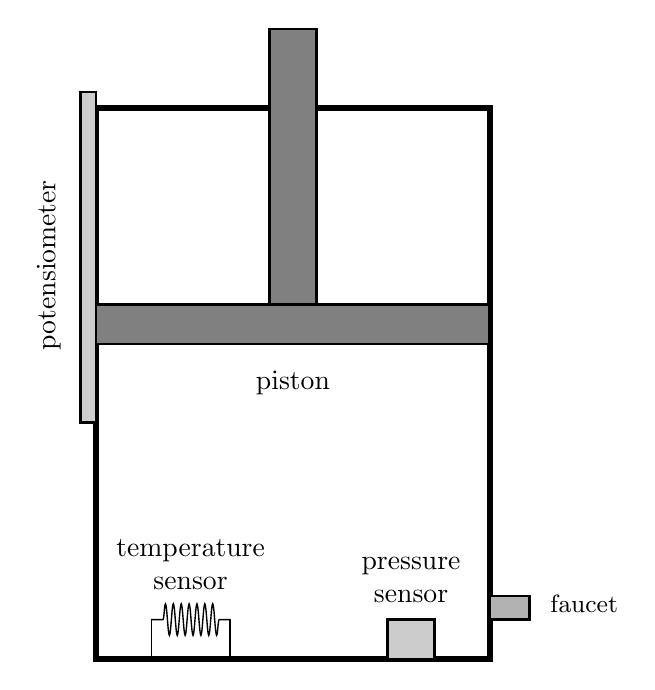
\begin{tikzpicture}
		% Grid
%		\foreach \i in {0,...,10}
%		{
%			\node at (-2ex,\i) {\i};
%			\node at (\i,-2ex) {\i};
%		}
		
		% Container
		\draw[line width=2] (3,2) rectangle (8,9);
		%% Piston
		\draw[line width =1, draw=black, fill=black!50] (3,6) rectangle (8,6.5);
		\draw[line width = 1, fill=black!50] (5.2,6.5) rectangle (5.8,10);
		%% Faucet
		\draw[line width=1, fill=black!30] (8,2.5) rectangle (8.5,2.8);
		%% Potentionmeter
		\draw[line width=1, fill = black!20] (3,9.2) rectangle (2.8,5);
		%% Temperature Sensor
		\draw[snake, line width=0.5] (3.7,2.5) -- (4.7,2.5);
		\draw[line width=0.5] (3.7,2.505) -- (3.7,2);
		\draw[line width=0.5] (4.7,2.505) -- (4.7,2);
		%% Pressure Sensor
		\draw[fill=black!20, line width=1] (6.7,2) rectangle (7.3,2.5);
		
		% Nodes
		\node at (5.5,5.5) {piston};
		\node[rotate=90] at (2.4,7) {potensiometer};
		\node at (4.2,3.2) {temperature\\sensor};
		\node at (7,3) {pressure\\sensor};
		\node at (9.2,2.7) {\small faucet};
	\end{tikzpicture}
	
\end{document}